% <!-- coding: utf-8 -->
\renewcommand{\monlhead}{Données serena}
\section{Données serena}
Les données sont extraites de serena

Cette extraction est faite en format xls. Les données sont ensuite traitées en R :
\begin{itemize}
\item suppression des données "Hors protocole"
\item normalisation du champ OBSE PLACE
\item détermination de la maille à partir du champ OBSE PLACE
\item détermination de la maille à partir des coordonnées géographiques
\end{itemize}

\subsection{par espèce}
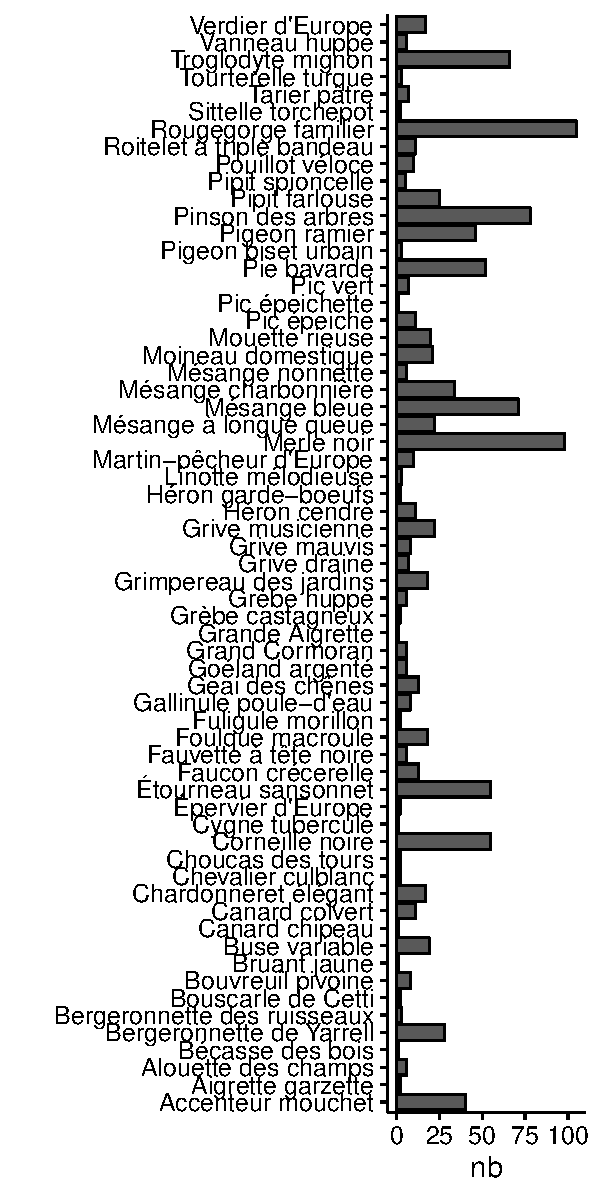
\includegraphics[width=\malargeurgraphique]{images/serena_stat_champ_espece.pdf}
\subsection{par date}
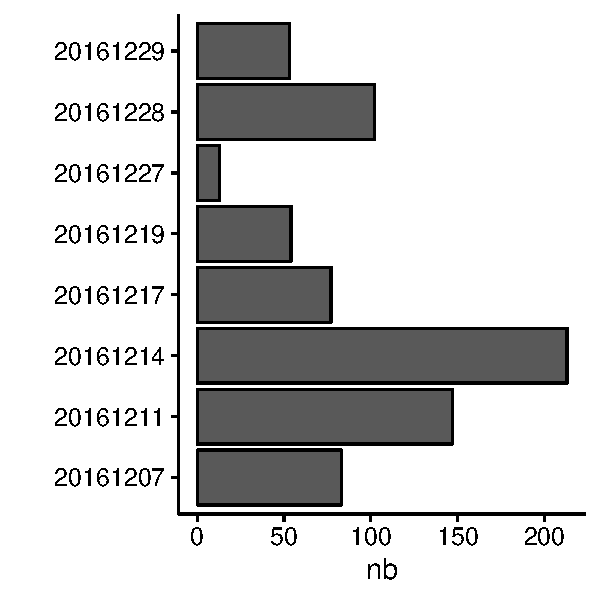
\includegraphics[width=\malargeurgraphique]{images/serena_stat_champ_OBSE_DATE.pdf}
\subsection{par observateur}
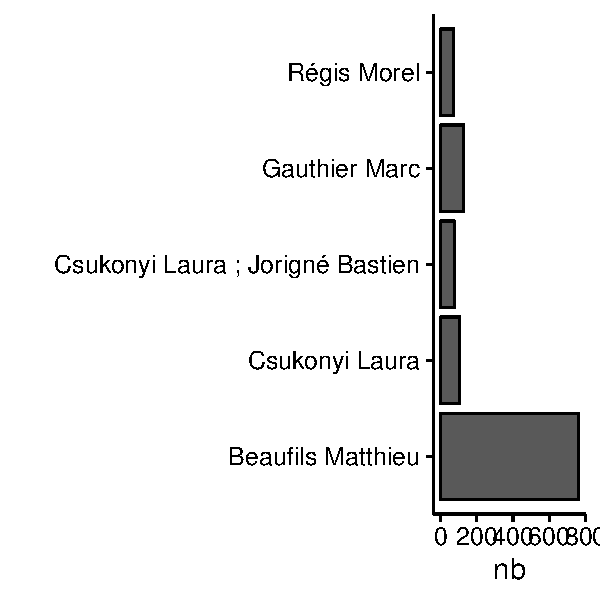
\includegraphics[width=\malargeurgraphique]{images/serena_stat_champ_OBSV_LIBEL.pdf}
\onecolumn
\subsection{carte parcours}
Le parcours est localisé en fonction de ses coordonnées.

En noir, les parcours avec une incohérence maille.
\begin{figure}[!h]
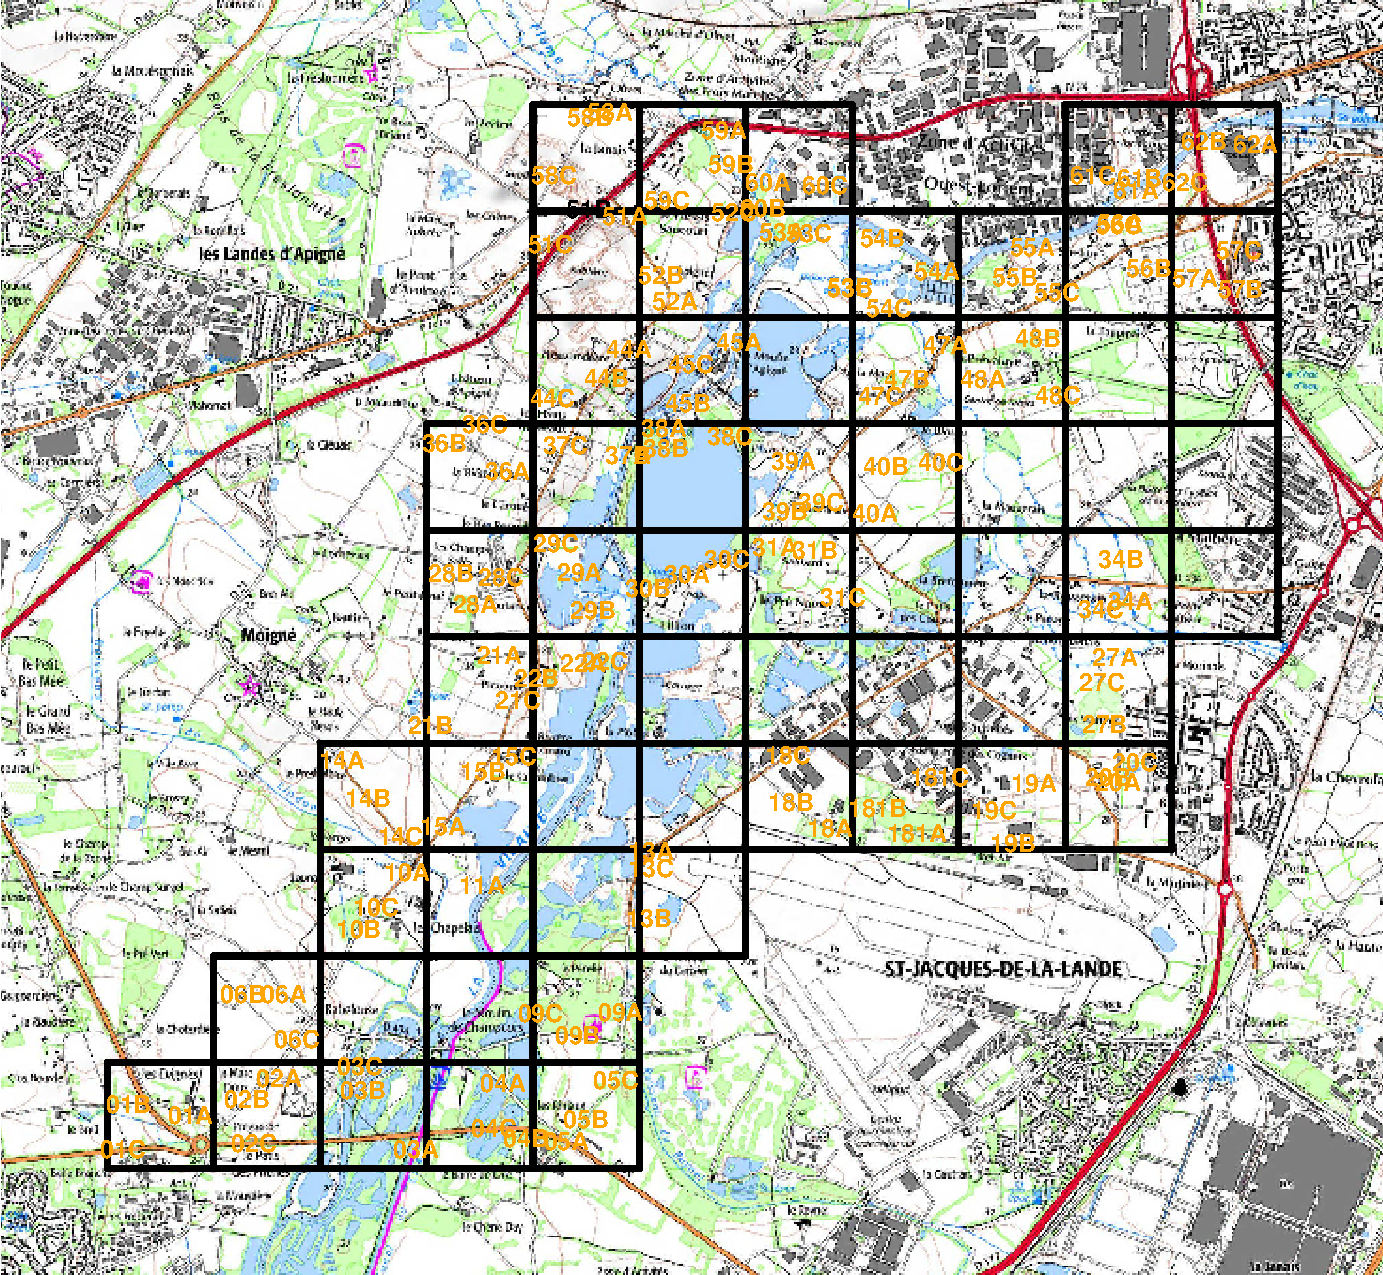
\includegraphics[width=1.0\textwidth]{images/serena_carte.pdf}
\end{figure}
\clearpage
\subsection{carte statistiques}
Pour chaque maille, on a le nombre de :
\begin{itemize}
\item parcours"
\item espèces
\item données
\end{itemize}
\begin{figure}[!h]
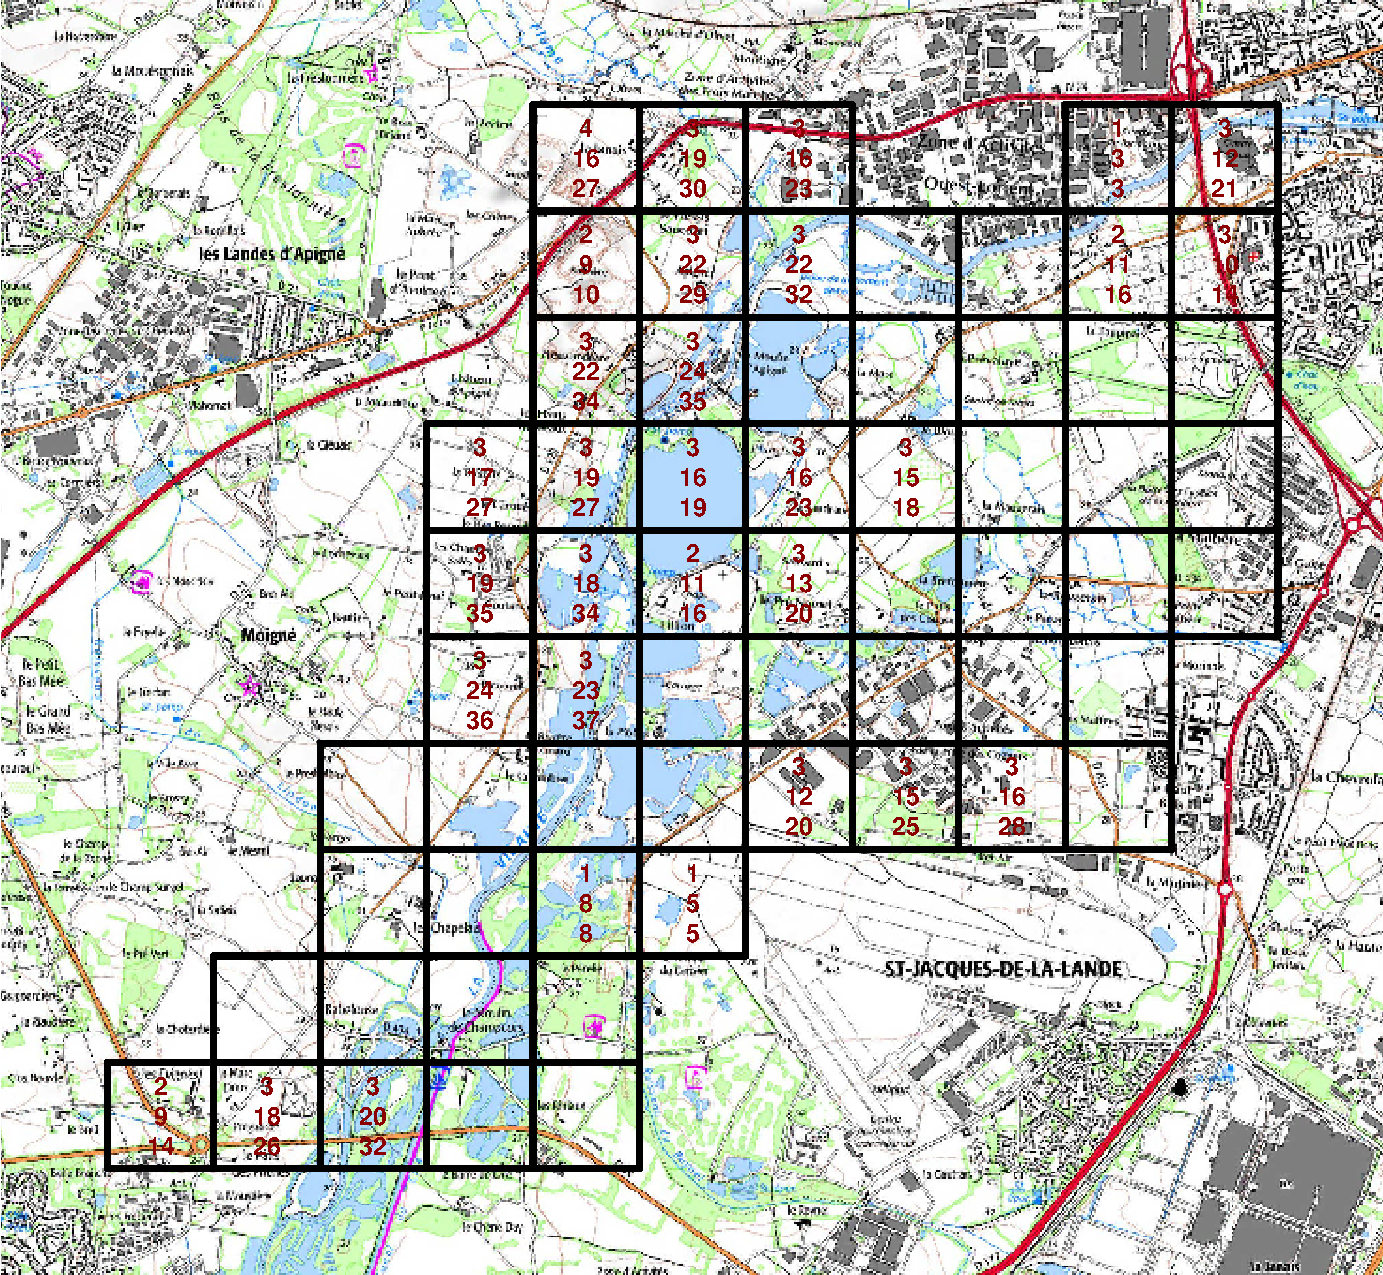
\includegraphics[width=1.0\textwidth]{images/serena_carte_stat.pdf}
\end{figure}
\clearpage
\twocolumn